\begin{enumerate}[label=\thechapter.\arabic*,ref=\thechapter.\theenumi]
\item The network shown below has a resonant frequency of 150 kHz and bandwidth of 600
Hz. The Q-factor of the network is \rule{1cm}{0.15mm}\\
(rounded off to one decimal place).\\
\hfill(GATE 2022 EC)\\
\begin{figure}[ht]
  \centering
  
      \begin{circuitikz}[american]
\draw (0,3) to [short,*-, i=$i_c$] (1,3) to [R=$R$] (4,3);
\draw (0,0) to [short, *-] (4,0);
\draw (4,3) to [short, i=$i_d$] (4,2.5) to [C=$C$] (4,0);
\end{circuitikz}
  
  \caption{Circuit 1}
\end{figure}\\
\solution\\
\iffalse
\let\negmedspace\undefined
\let\negthickspace\undefined
\documentclass[journal,12pt,twocolumn]{IEEEtran}
\usepackage{cite}
\usepackage{amsmath,amssymb,amsfonts,amsthm}
\usepackage{algorithmic}
\usepackage{graphicx}
\usepackage{textcomp}
\usepackage{xcolor}
\usepackage{txfonts}
\usepackage{listings}
\usepackage{enumitem}
\usepackage{mathtools}
\usepackage{gensymb}
\usepackage{comment}
\usepackage[breaklinks=true]{hyperref}
\usepackage{tkz-euclide} 
\usepackage{listings}
\usepackage{gvv}                                        
\def\inputGnumericTable{}                                 
\usepackage[latin1]{inputenc}                                
\usepackage{color}                                            
\usepackage{array}                                            
\usepackage{longtable}                                       
\usepackage{calc}                                             
\usepackage{multirow}                                         
\usepackage{hhline}                                           
\usepackage{ifthen}                                           
\usepackage{lscape}
\usepackage[center]{caption} % center the captions to figure

\newtheorem{theorem}{Theorem}[section]
\newtheorem{problem}{Problem}
\newtheorem{proposition}{Proposition}[section]
\newtheorem{lemma}{Lemma}[section]
\newtheorem{corollary}[theorem]{Corollary}
\newtheorem{example}{Example}[section]
\newtheorem{definition}[problem]{Definition}
\newcommand{\BEQA}{\begin{eqnarray}}
\newcommand{\EEQA}{\end{eqnarray}}
\newcommand{\define}{\stackrel{\triangle}{=}}
\theoremstyle{remark}
\newtheorem{rem}{Remark}
\begin{document}

\newcolumntype{M}[1]{>{\centering\arraybackslash}m{#1}}
\newcolumntype{N}{@{}m{0pt}@{}}

\bibliographystyle{IEEEtran}
\vspace{3cm}

\title{GATE 2022 BM 14 Q} 
\author{ee23btech11223 - Soham Prabhakar More% <-this % stops a space
}
\maketitle
\newpage
\bigskip

\renewcommand{\thefigure}{\theenumi}
\renewcommand{\thetable}{\theenumi}

\bibliographystyle{IEEEtran}

\textbf{Question:} $x\brak{t}$ is a real continuous-time signal whose magnitude frequency response
$\abs{X\brak{j\Omega}}$ is shown below. After sampling $x\brak{t}$ at 100 $rad.s^{-1}$, the spectral point P
is down-converted to \rule{1cm}{0.15mm} $rad.s^{-1}$ in the spectrum of the sampled signal.
\hfill{(GATE 2022 BM 14 Q)}
\begin{figure}[h!]
    \renewcommand\thefigure{1}
    \centering
    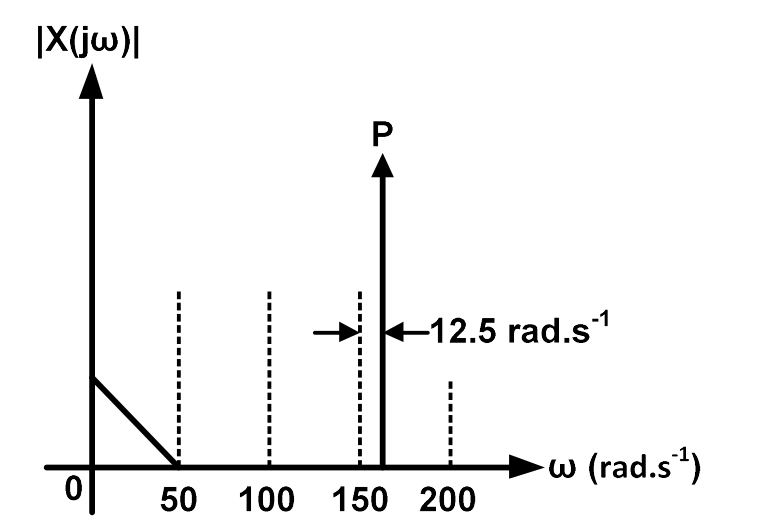
\includegraphics[width=\columnwidth]{2022/BM/14/figs/question.png}
    \caption[short]{Plot of $\abs{X\brak{j\omega}}$}
    \label{fig:2023.bm.14.img1}
\end{figure}

\solution
\fi
\begin{table}[ht]
    \renewcommand\thetable{1}
\begin{tabular}{|c|c|}
    \hline 
    \textbf{Parameter}&\textbf{Description} \\
    \hline
    $w\brak{t}$ & Sampling Function \\
    \hline
	$W\brak{j\omega}$ & Fourier Transform of $w\brak{t}$ \\
    \hline
    $x\brak{t}$ & Input Signal \\
    \hline
    $X\brak{j\omega}$ & Input Signal Frequency Spectrum \\
    \hline
    $x_s\brak{t}$ & Sampled Input Signal \\
    \hline
    $X_s\brak{j\omega}$ & Sampled Signal Frequency Spectrum \\
    \hline
\end{tabular}

\caption{Table of parameters}
\label{Table:1}


\end{table} \\
The sampling function is:
\begin{align}
    w(t) &= \sum_{k = -\infty}^{\infty}\delta\brak{t - \frac{2\pi k}{100}} \\
    W(j\omega) &= 100\sum_{k = -\infty}^{\infty}\delta\brak{j\brak{\omega - 100k}}
\end{align}
then the sampled function: 
\begin{align}
    x_s\brak{t} &= x\brak{t}w\brak{t} \\
    X_s\brak{j\omega} &= X\brak{j\omega} * W\brak{j\omega} \\
    X_s\brak{j\omega} &= \int_{-\infty}^{\infty}X\brak{j\theta}W\brak{j\brak{\omega - \theta}}d\theta \\
    X_s\brak{j\omega} &= 100\sum_{k = -\infty}^{\infty}\int_{-\infty}^{\infty}X\brak{j\theta}\delta\brak{j\brak{\omega - 100k - \theta}}d\theta \\
    X_s\brak{j\omega} &= 100\sum_{k = -\infty}^{\infty}X\brak{j\brak{\omega - 100k}} 
\end{align}
Thus, The down sampled point is at:
\begin{align}
    \omega &= \abs{162.5 - 100k}
\end{align}
where $k$ is the nearest integer to $\frac{162.5}{100}$, which is 2\\
Thus,
\begin{align}
    \omega = 37.5\,rad\,s^{-1}
\end{align}

\begin{figure}[h!]
    \renewcommand\thefigure{2}
    \centering
    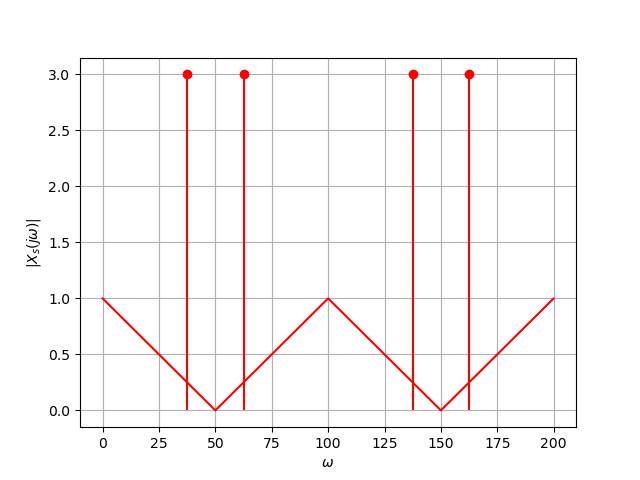
\includegraphics[width=\columnwidth]{2022/BM/14/figs/X_s.png}
    \caption[short]{Plot of $\abs{X_s\brak{j\omega}}$}
    \label{fig:2023.bm.14.img2}
\end{figure}

%\end{document}

\pagebreak
\item A circuit with an ideal OPAMP is shown. The Bode plot for the magnitude (in dB)
 of the gain transfer function $ \brak{A \brak{j \omega}} = \dfrac{ V_{out}\brak{j \omega}}{V_{in}\brak{j \omega}}$ of the circuit is also
provided (here, $\omega$ is the angular frequency in $ rad/s $). The values of $R$ and $C$ are 
\begin{figure}[ht]
	\centering
    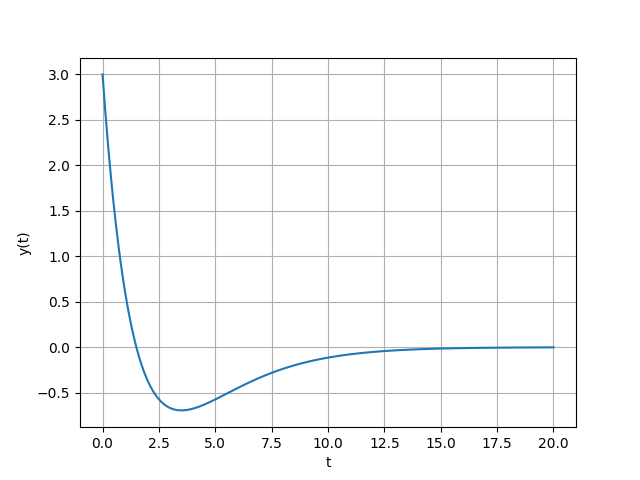
\includegraphics[width=\columnwidth]{2022/EC/42/figs/fig1.png}
    \label{fig:2022.42.39}
\end{figure} 
\begin{enumerate}[label = (\Alph*)]
     \item $R$ = $3k\ohm$,  $C$ = $1\mu F$\\
     \item $R$ = $1k\ohm$,  $C$ = $3\mu F$\\
     \item $R$ = $4k\ohm$,  $C$ = $1\mu F$\\
     \item $R$ = $3k\ohm$,  $C$ = $2\mu F$\\
\end{enumerate}
\hfill(GATE 2022 EC)\\
\solution\\
\input{2022/EC/42/ec.tex}
\pagebreak

\item  In the circuit shown, the load is driven by a sinusoidal A.C. voltage source $V_1 = 100\angle0\degree V$ at $50Hz$. Given $R_1 = 20\Omega$, $C_1 = \brak{\frac{1000}{\pi}}\mu F$, $L_1 = \brak{\frac{20}{\pi}}mH$ and $R_2 = 4\Omega$, the power factor is \_\_\_\_\_ (round off to one decimal place)\\
\hfill(GATE 2022 IN Q52)
\begin{figure}[!h]
    \centering
    \begin{circuitikz}
        \draw(0, 0) to[sV, l = $V_1$](0, -4);
        \draw(0, -4) to [R, l = $R_2$](6, -4);
        \draw(6, 0) to[L, l = $L_1$](6, -4);
        \draw(0, 0) -- (2, 0);
        \draw(4, 0) -- (6, 0);
        \draw(2, 0.75) -- (2, -0.75);
        \draw(4, 0.75) -- (4, -0.75);

        \draw(2, 0.75) to [R, l = $R_1$](4, 0.75);
        \draw(2, -0.75) to [C, l_ = $C_1$](4, -0.75);
    \end{circuitikz}
    \caption{}
    \label{fig:1_gate.22.in.52}
\end{figure}

\solution
\iffalse
\let\negmedspace\undefined
\let\negthickspace\undefined
\documentclass[journal,12pt,twocolumn]{IEEEtran}
\usepackage{cite}
\usepackage{amsmath,amssymb,amsfonts,amsthm}
\usepackage{algorithmic}
\usepackage{graphicx}
\usepackage{textcomp}
\usepackage{xcolor}
\usepackage{txfonts}
\usepackage{listings}
\usepackage{enumitem}
\usepackage{mathtools}
\usepackage{gensymb}
\usepackage{comment}
\usepackage[breaklinks=true]{hyperref}
\usepackage{tkz-euclide} 
\usepackage{listings}
\usepackage{gvv}                            \usepackage{tikz}
\usepackage{circuitikz}
\def\inputGnumericTable{}                                
\usepackage[latin1]{inputenc}                            
\usepackage{color}                      \usepackage{gensymb}
\usepackage{array}                                       
\usepackage{longtable}                                   
\usepackage{calc}                              
\usepackage{tikz}
\usepackage{multirow}                                    
\usepackage{hhline}                                      
\usepackage{ifthen}                            
\usepackage{caption}
\usepackage{lscape}
\usepackage{amsmath}
\newtheorem{theorem}{Theorem}[section]
\newtheorem{problem}{Problem}
\newtheorem{proposition}{Proposition}[section]
\newtheorem{lemma}{Lemma}[section]
\newtheorem{corollary}[theorem]{Corollary}
\newtheorem{example}{Example}[section]
\newtheorem{definition}[problem]{Definition}
\newcommand{\BEQA}{\begin{eqnarray}}
\newcommand{\EEQA}{\end{eqnarray}}
\newcommand{\define}{\stackrel{\triangle}{=}}
\theoremstyle{remark}
\newtheorem{rem}{Remark}

\begin{document}

\bibliographystyle{IEEEtran}
\vspace{3cm}

\title{GATE 2022 IN Q52}
\author{EE23BTECH11009 - AROSHISH PRADHAN$^{*}$% <-this % stops a space
}
\maketitle
\newpage
\bigskip
\textbf{Question:} In the circuit shown, the load is driven by a sinusoidal A.C. voltage source $V_1 = 100\angle0\degree V$ at $50Hz$. Given $R_1 = 20\Omega$, $C_1 = \brak{\frac{1000}{\pi}}\mu F$, $L_1 = \brak{\frac{20}{\pi}}mH$ and $R_2 = 4\Omega$, the power factor is \_\_\_\_\_ (round off to one decimal place)\\
\hfill(GATE 2022 IN Q52)
\begin{figure}[!h]
    \centering
    \begin{circuitikz}
        \draw(0, 0) to[sV, l = $V_1$](0, -4);
        \draw(0, -4) to [R, l = $R_2$](6, -4);
        \draw(6, 0) to[L, l = $L_1$](6, -4);
        \draw(0, 0) -- (2, 0);
        \draw(4, 0) -- (6, 0);
        \draw(2, 0.75) -- (2, -0.75);
        \draw(4, 0.75) -- (4, -0.75);

        \draw(2, 0.75) to [R, l = $R_1$](4, 0.75);
        \draw(2, -0.75) to [C, l_ = $C_1$](4, -0.75);
    \end{circuitikz}
    \caption{}
    \label{fig:1_gate.22.in.52}
\end{figure}


\solution
\fi
\begin{table}[!h]
    \centering
    \begin{tabular}{|c|c|c|}
    \hline
       \textbf{Symbol}  & \textbf{Value}  & \textbf{Description}\\
    \hline
       $V_1$  & $100\angle0\degree V$ & Input Voltage \\
    \hline
        $f$ & $50Hz$ & Frequency\\
    \hline
        $\omega$ & $2\pi f$ & Angular Frequency\\
    \hline
        $R_1$ & $20\Omega$ & Resistance\\
    \hline
        $R_2$ & $4\Omega$ & Resistance\\
    \hline
        $C_1$ & $\brak{\frac{1000}{\pi}}\mu F$ & Capacitance\\
    \hline
        $L_1$ & $\brak{\frac{20}{\pi}}mH$ & Inductance\\
    \hline
        $Z_{\text{eff}}$ & & Impedance\\
    \hline
        $\cos(\phi)$ & $\dfrac{\mathrm{Re}(Z_{\text{eff}})}{\abs{Z_{\text{eff}}}}$& Power Factor\\
    \hline
    \end{tabular}
    \caption{Given Parameters}
    \label{tab:1_gate.22.in.52}
\end{table}


\begin{align}
    Z_{\text{eff}} &= R_2 + j\omega L_1 + \frac{\frac{R_1}{j\omega C_1}}{R_1 + \frac{1}{j\omega C_1}}\\
    &= 4 + 2j + \frac{-200j}{20 - 10j}\\
    &= 8-6j
\end{align}
$\therefore$ Power Factor:
\begin{align}
    \cos(\phi) &= \frac{\mathrm{Re}(Z_{\text{eff}})}{\abs{Z_{\text{eff}}}}\\
    &= \frac{8}{\sqrt{8^2 + 6^2}}\\
    &= 0.8
\end{align}
\begin{figure}[!h]
    \centering
    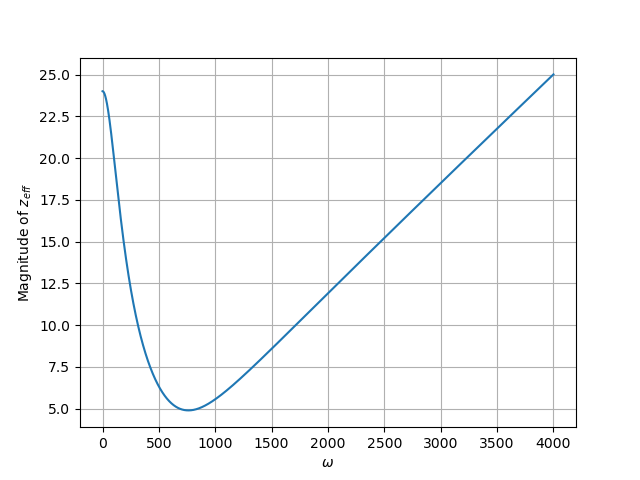
\includegraphics[width = \columnwidth]{2022/IN/52/figs/Zplot.png}
    \caption{Plot of $Z_{\text{eff}}$ vs $\omega$}
    \label{fig:2_gate.22.in.52}
\end{figure}
%\end{document}

\pagebreak

\item For the circuit shown, the locus of the impedance $ Z\brak{j\omega}$ is plotted as $ \omega$ increases from zero to infinity. The values of $ R_1$ and $ R_2$ are:
\begin{enumerate}
    \item[(A)] $ R_1 = 2\text{ k\ohm}, R_2 = 3\text{ k\ohm}$
    \item[(B)]$ R_1 = 5\text{ k\ohm}, R_2 = 2\text{ k\ohm}$
    \item[(C)] $ R_1 = 5\text{ k\ohm}, R_2 = 2.5\text{ k\ohm}$
    \item[(D)] $ R_1 = 2\text{ k\ohm}, R_2 = 5\text{ k\ohm}$
\end{enumerate}

\begin{figure}[h!]
    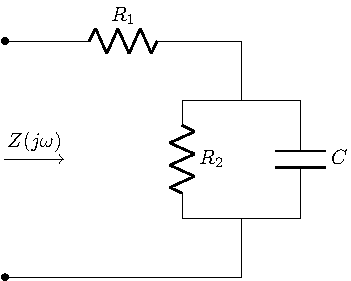
\includegraphics[width = 0.6\columnwidth]{2022/EC/38/figs/qn_fig.pdf}
    \caption{Figure of circuit}
    \centering
    \label{fig: ece38_qn_fig}
\end{figure}

\begin{figure}[h!]
    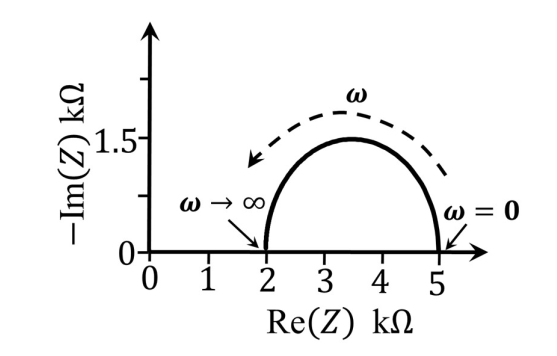
\includegraphics[width = 0.6\columnwidth]{2022/EC/38/figs/fig_2.png}
    \caption{}
    \centering
    \label{fig: ece38qn_2_fig}
\end{figure}
\hfill(GATE ECE 2022 QUESTION 38)\\
\solution
 \iffalse
\let\negmedspace\undefined
\let\negthickspace\undefined
\documentclass[journal,12pt,twocolumn]{IEEEtran}
\usepackage{cite}
\usepackage{amsmath,amssymb,amsfonts,amsthm}
\usepackage{algorithmic}
\usepackage{graphicx}
\usepackage{textcomp}
\usepackage{xcolor}
\usepackage{txfonts}
\usepackage{listings}
\usepackage{enumitem}
\usepackage{mathtools}
\usepackage{gensymb}
\usepackage{comment}
\usepackage[breaklinks=true]{hyperref}
\usepackage{tkz-euclide}
\usepackage{listings}
\usepackage{gvv}
\def\inputGnumericTable{}
\usepackage[latin1]{inputenc}
\usepackage{color}
\usepackage{array}
\usepackage{longtable}
\usepackage{calc}
\usepackage{multirow}
\usepackage{hhline}
\usepackage{ifthen}
\usepackage{lscape}

\newtheorem{theorem}{Theorem}[section]
\newtheorem{problem}{Problem}
\newtheorem{proposition}{Proposition}[section]
\newtheorem{lemma}{Lemma}[section]
\newtheorem{corollary}[theorem]{Corollary}
\newtheorem{example}{Example}[section]
\newtheorem{definition}[problem]{Definition}
\newcommand{\BEQA}{\begin{eqnarray}}
\newcommand{\EEQA}{\end{eqnarray}}
\newcommand{\define}{\stackrel{\triangle}{=}}
\theoremstyle{remark}
\newtheorem{rem}{Remark}
\begin{document}

\bibliographystyle{IEEEtran}
\vspace{3cm}

\title{GATE 2022  -AE 63}
\author{EE23BTECH11057 - Shakunaveti Sai Sri Ram Varun$^{}$% &lt;-this % stops a space
}
\maketitle
\newpage
\bigskip
\vspace{2cm}
\textbf{Question: }
For the circuit shown, the locus of the impedance $ Z\brak{j\omega}$ is plotted as $ \omega$ increases from zero to infinity. The values of $ R_1$ and $ R_2$ are:
\begin{enumerate}
    \item[(A)] $ R_1 = 2\text{ k\ohm}, R_2 = 3\text{ k\ohm}$
    \item[(B)]$ R_1 = 5\text{ k\ohm}, R_2 = 2\text{ k\ohm}$
    \item[(C)] $ R_1 = 5\text{ k\ohm}, R_2 = 2.5\text{ k\ohm}$
    \item[(D)] $ R_1 = 2\text{ k\ohm}, R_2 = 5\text{ k\ohm}$
\end{enumerate}

\begin{figure}[h!]
    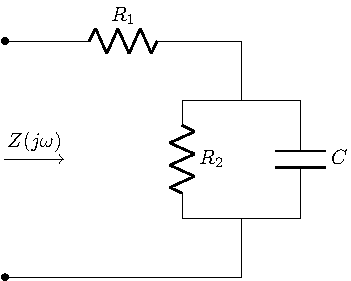
\includegraphics[width = 0.6\columnwidth]{2022/EC/38/figs/qn_fig.pdf}
    \caption{Figure of circuit}
    \centering
    \label{fig: ece38_qn_fig}
\end{figure}

\begin{figure}[h!]
    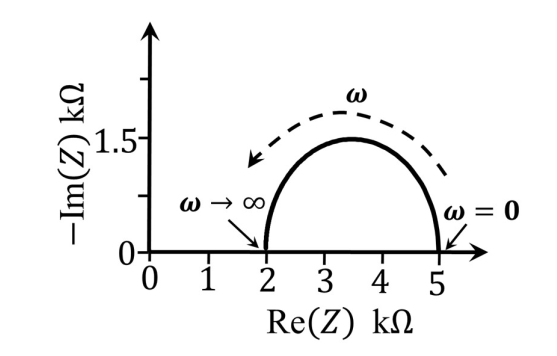
\includegraphics[width = 0.6\columnwidth]{2022/EC/38/figs/fig_2.png}
    \caption{}
    \centering
    \label{fig: ece38qn_2_fig}
\end{figure}
\hfill(GATE ECE 2022 QUESTION 38)\\
\textbf{Solution}:\\
\fi
\begin{table}[h!] 
\centering
\begin{tabular}{|c|c|c|}
    \hline
    \textbf{Parameter} & \textbf{Description} & \textbf{Value} \\
    \hline
    $ Z\brak{j\omega}$ & Impedance of circuit & ? \\
    \hline
    $ R_1$ & Resistor 1  &? \\
    \hline
    $ R_1$ & Resistor 2  &? \\
    \hline
    $ C$ & Capacitor  &? \\
    \hline
    $\omega$ & angular frequency of input voltage& $ \omega$\\
    \hline
\end{tabular}





\caption{input values}
\label{tab: Table2022ECE38}
\end{table}

In $ \omega$ domain (i.e. after Laplace transform) \figref{fig: ece38_qn_fig} can be represented as \figref{fig: ece38_ans_1_fig}
\begin{figure}[h!]
    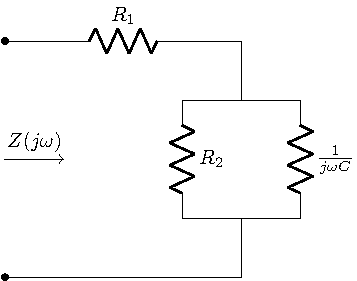
\includegraphics[width = 0.6\columnwidth]{2022/EC/38/figs/answer_fig.pdf}
    \caption{}
    \centering
    \label{fig: ece38_ans_1_fig}
\end{figure}
So, the impedance for the circuit in $ \omega$ domain is:
\begin{align}
Z\brak{j \omega} &= R_1 +  \frac{1}{\frac{1}{R_2}+ j\omega C} \label{eq: ece38_1}
\end{align}
From \figref{fig: ece38qn_2_fig}, $ Z\brak{j\omega}=2$ as $ \omega \to \infty$ and 
$ Z\brak{j\omega}=5$ as $ \omega \to 0$
\begin{align}
2 &= R_1 + \lim_{\omega\to\infty}\frac{1}{\frac{1}{R_2}+ j\omega C}\\
\implies 2 &= R_1 + \lim_{\omega\to\infty}\frac{\frac{1}{R_2}- j \omega C}{\brak{\frac{1}{R_2}}^2+ \brak{\omega C}^2}\\
\implies 2 &= R_1 + \lim_{\omega\to\infty}\frac{\frac{1}{R_2 \omega^2}- j\frac{C}{\omega}}{\brak{\frac{1}{R_2 \omega}}^2+ C^2}\\
\therefore R_1 \label{eq: ece_38_2}&= 2\text{\ohm}\\
5 &= R_1 + \frac{1}{\frac{1}{R_2}+j\brak{0}}\\
\implies 5 &= R_1 + R_2\\
\therefore R_2 &= 3\text{\ohm} 
\end{align}
Hence, option (A) is correct.


\pagebreak

\item In the bandpass filter circuit shown, $R_0 = 50\Omega$, $L_0 = 1 mH$, $C_0 = 10nF$. The q factor of the filter is 
\begin{figure}[h]
\renewcommand\thefigure{1}
    \centering
    \begin{circuitikz}[american]
    \draw (0,0) to [L=$L_0$, *-] (2,0) to [C=$C_0$] (4,0) to [R=$R_0$] (4,-2) to [short, -*] (0,-2);
    \draw (4,-0.3) to[short, -*] (6,-0.3);
    \draw (4,-1.7) to[short, -*] (6,-1.7);

    \node at (6,-1) {Output};
    \node at (0,-1) {Input};
    \end{circuitikz}
\end{figure}


\hfill(GATE 2022 IN Q33)\\
\solution
\iffalse
\let\negmedspace\undefined
\let\negthickspace\undefined
\documentclass[journal,12pt,twocolumn]{IEEEtran}
\usepackage{cite}
\usepackage{circuitikz}
\usepackage{amsmath,amssymb,amsfonts,amsthm}
\usepackage{algorithmic}
\usepackage{graphicx}
\usepackage{textcomp}
\usepackage{xcolor}
\usepackage{txfonts}
\usepackage{listings}
\usepackage{enumitem}
\usepackage{mathtools}
\usepackage{gensymb}
\usepackage{comment}
\usepackage[breaklinks=true]{hyperref}
\usepackage{tkz-euclide} 
\usepackage{listings}
\usepackage{gvv}                                        
\def\inputGnumericTable{}                                 
\usepackage[latin1]{inputenc}                                
\usepackage{color}                                            
\newtheorem{theorem}{Theorem}[section]
\usepackage{array}                                            
\usepackage{longtable}                                       
\usepackage{calc}                                             
\usepackage{multirow}                                         
\usepackage{hhline}                                           
\usepackage{ifthen}                                           
\usepackage{lscape}
\newtheorem{problem}{Problem}
\newtheorem{proposition}{Proposition}[section]
\newtheorem{lemma}{Lemma}[section]
\newtheorem{corollary}[theorem]{Corollary}
\newtheorem{example}{Example}[section]
\newtheorem{definition}[problem]{Definition}
\newcommand{\BEQA}{\begin{eqnarray}}
\newcommand{\EEQA}{\end{eqnarray}}
\newcommand{\define}{\stackrel{\triangle}{=}}
\theoremstyle{remark}
\newtheorem{rem}{Remark}
\begin{document}
\bibliographystyle{IEEEtran}
\vspace{3cm}
\title{GATE 22 IN/33}
\author{EE23BTECH11040 - Manoj Kumar Ambatipudi$^{*}$% <-this % stops a space
}
\maketitle
\newpage
\bigskip
\renewcommand{\thefigure}{\theenumi}
\renewcommand{\thetable}{\theenumi}
\textbf{QUESTION:}
In the bandpass filter circuit shown, $R_0 = 50\Omega$, $L_0 = 1 mH$, $C_0 = 10nF$. The q factor of the filter is 
\begin{figure}[h]
\renewcommand\thefigure{1}
    \centering
    \begin{circuitikz}[american]
    \draw (0,0) to [L=$L_0$, *-] (2,0) to [C=$C_0$] (4,0) to [R=$R_0$] (4,-2) to [short, -*] (0,-2);
    \draw (4,-0.3) to[short, -*] (6,-0.3);
    \draw (4,-1.7) to[short, -*] (6,-1.7);

    \node at (6,-1) {Output};
    \node at (0,-1) {Input};
    \end{circuitikz}
\end{figure}


\solution
\fi
\begin{table}[h]
\renewcommand\thetable{1}
    \centering
    \begin{tabular}{|c|c|c|}
    \hline
     Variable & Description&Value\\\hline
        $R_0$ & Resistance & $50\Omega$ \\\hline
        $L_0$ & Inductance & $1mH$ \\\hline
        $C_0$ & Capacitance & $10nF$\\\hline
        $\omega_0$& Resonant Angular Frequency & $\frac{1}{\sqrt{L_0C_0}}$\\\hline
    \end{tabular}
    \caption{Variables and their description}
    \label{tab_22_33_1}
\end{table}
\\
The corresponding Laplace domain circuit is 
\begin{figure}[h]
\renewcommand\thefigure{2}
    \centering
    \begin{circuitikz}[american]
    \draw (0,0) to [generic=$sL_0$, *-] (2,0) to [generic=$\frac{1}{sC_0}$] (4,0) to [generic=$R_0$] (4,-2) to [short, -*] (0,-2);
    \draw (4,-0.3) to[short, -*] (6,-0.3);
    \draw (4,-1.7) to[short, -*] (6,-1.7);
    \node at (6,-1) {Output};
    \node at (0,-1) {Input};
    \end{circuitikz}
\end{figure}


Input $X\brak{s}$ can be written as
\begin{align}
    X\brak{s} = I\brak{s}\brak{sL_0 + \frac{1}{sC_0} + R_0} 
\end{align}
Output $Y\brak{s}$ can be written as 
\begin{align}
    Y\brak{s} = I\brak{s}R_0
\end{align}
Transfer function $H\brak{s}$ can be written as 
\begin{align}
    H\brak{s} &= \frac{Y\brak{s}}{X\brak{s}}\\ &= \frac{sC_0R_0}{s^2C_0L_0 + C_0R_0s + 1}
\end{align}
substituting $s = j\omega$
\begin{align}
    H\brak{j,\omega} = \frac{j\omega C_0R_0}{-\omega^2C_0L_0 + jC_0R_0\omega + 1}\\
\implies \abs{H\brak{j,\omega}} = \frac{\omega C_0R_0}{\sqrt{\brak{1-\omega^2C_0L_0}^2 + \brak{C_0R_0\omega}^{2}}}
\end{align}
Differentiating w.r.t $\omega$ and equating to 0, we get 
\begin{align}
    \frac{d\abs{H\brak{j,\omega}}}{d\omega} &= \frac{C_0R_0}{\sqrt{\brak{1-\omega^2C_0L_0}^2 + \brak{C_0R_0\omega}^{2}}} +\notag\\& \frac{\omega C_0R_0}{2\brak{\brak{1-\omega^2C_0L_0}^2 + \brak{C_0R_0\omega}^{2}}^{\frac{3}{2}}}\notag\\&\brak{2\omega\brak{C_0R_0}^2-2\brak{1-\omega^2C_0L_0}2\omega} &= 0\\
    \implies \omega_0 &= \frac{1}{\sqrt{L_0C_0}}\label{eq_22_33_1}
\end{align}
from \tabref{tab_22_33_1}, 
\begin{align}
    \omega_0 = 316227.76
\end{align}
$Q-factor$ defined with reference to inductor
\begin{align}
    Q &= \abs{\frac{V_L}{V_R}}_{\omega_0}\\
      &= \frac{L_0\omega_0}{R_0}\\
      &= \frac{1}{R_0}\sqrt{\frac{L_0}{C_0}} \quad\brak{\text{from \eqref{eq_22_33_1}}}
\end{align}
$Q-factor$ defined with reference to capacitor
\begin{align}
    Q &= \abs{\frac{V_C}{V_R}}_{\omega_0}\\
      &= \frac{1}{C_0\omega_0R_0}\\
      &= \frac{1}{R_0}\sqrt{\frac{L_0}{C_0}} \quad\brak{\text{from \eqref{eq_22_33_1}}}
\end{align}
Substituting the values from \tabref{tab_22_33_1}, we get
\begin{align}
    Q = 200
\end{align}
\begin{figure}
\renewcommand\thefigure{1}
    \centering
    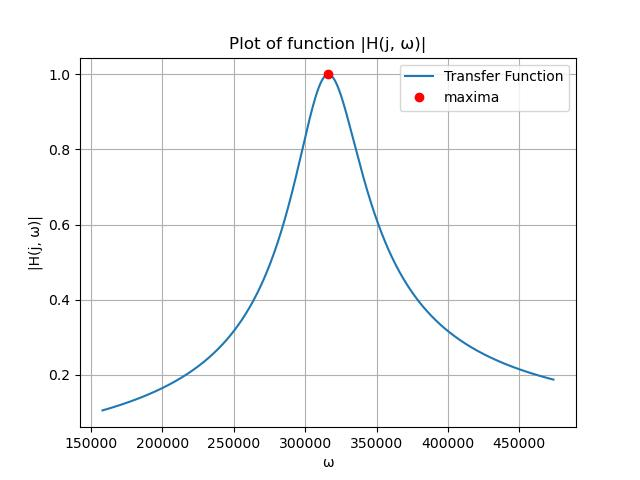
\includegraphics[width=1.0\columnwidth]{2022/IN/33/figs/fig_1.jpg}
    \caption{Transfer function $\abs{H\brak{j, \omega}}$ taken from python3}
\end{figure}

\pagebreak

\item In the circuit shown below, the switch S is closed at $t=0$. The magnitude of the steady state voltage, in volts, across the $6\Omega$ resistor is \_\_\_\_\_.(\textit{round off to two decimal places})\\ \hfill(GATE 2022 EE Q31)
\begin{figure}[!h]
    \centering
    \begin{circuitikz}[scale = 0.8]
        \draw(0, 0) -- (1, 0);
        \draw(1, 0.5) -- (1, -0.5);
        \draw(4, 0.5) -- (4, -0.5);
        \draw(4, 0) -- (5, 0);

        \draw(1, 0.5) to[R, l = $6\Omega$](4, 0.5);
        \draw(1, -0.5) to[R, l_ = $3\Omega$](4, -0.5);

        \draw(0, 0) -- (0, -2);
        \draw(5, 0) -- (5, -2);

        \draw(0, -2) to[C, l = $1\mu F$](2, -2);
        \draw(2, -2) to [R, l = $10\Omega$](5, -2);

        \draw(0, -2) -- (0, -3.5);
        \draw(5, -2) -- (5, -3.5);

        \draw(0, -3.5) to[battery2, l_ = $10V$](1.5, -3.5);
        \draw (1.5, -3.5) to[switch, l = S] (2, -3.5);
        \draw(2, -3.5) to [R, l = $2\Omega$](5, -3.5);

        \draw[->](0, -3.5) -- (0, -2.5) node[midway, left] {$I$}; 
    \end{circuitikz}
    \caption{}
    \label{fig:1_gate.ee.22.31}
\end{figure}\\
\solution
\iffalse
\let\negmedspace\undefined
\let\negthickspace\undefined
\documentclass[journal,12pt,twocolumn]{IEEEtran}
\usepackage{cite}
\usepackage{amsmath,amssymb,amsfonts,amsthm}
\usepackage{algorithmic}
\usepackage{graphicx}
\usepackage{textcomp}
\usepackage{xcolor}
\usepackage{txfonts}
\usepackage{listings}
\usepackage{enumitem}
\usepackage{mathtools}
\usepackage{gensymb}
\usepackage{comment}
\usepackage[breaklinks=true]{hyperref}
\usepackage{tkz-euclide} 
\usepackage{listings}
\usepackage{gvv}                            \usepackage{tikz}
\usepackage{circuitikz}
\def\inputGnumericTable{}                                
\usepackage[latin1]{inputenc}                            
\usepackage{color}                                       
\usepackage{array}                                       
\usepackage{longtable}                                   
\usepackage{calc}                              
\usepackage{tikz}
\usepackage{multirow}                                    
\usepackage{hhline}                                      
\usepackage{ifthen}                            
\usepackage{caption}
\usepackage{lscape}
\usepackage{amsmath}
\newtheorem{theorem}{Theorem}[section]
\newtheorem{problem}{Problem}
\newtheorem{proposition}{Proposition}[section]
\newtheorem{lemma}{Lemma}[section]
\newtheorem{corollary}[theorem]{Corollary}
\newtheorem{example}{Example}[section]
\newtheorem{definition}[problem]{Definition}
\newcommand{\BEQA}{\begin{eqnarray}}
\newcommand{\EEQA}{\end{eqnarray}}
\newcommand{\define}{\stackrel{\triangle}{=}}
\theoremstyle{remark}
\newtheorem{rem}{Remark}

\begin{document}

\bibliographystyle{IEEEtran}
\vspace{3cm}

\title{GATE 2023 PH Q37}
\author{EE23BTECH11009 - AROSHISH PRADHAN$^{*}$% <-this % stops a space
}
\maketitle
\newpage
\bigskip
\textbf{Question:} In the circuit shown below, the switch S is closed at $t=0$. The magnitude of the steady state voltage, in volts, across the $6\Omega$ resistor is \_\_\_\_\_.(\textit{round off to two decimal places})\\ \hfill(GATE 2022 EE Q31)
\begin{figure}[!h]
    \centering
    \begin{circuitikz}[scale = 0.8]
        \draw(0, 0) -- (1, 0);
        \draw(1, 0.5) -- (1, -0.5);
        \draw(4, 0.5) -- (4, -0.5);
        \draw(4, 0) -- (5, 0);

        \draw(1, 0.5) to[R, l = $6\Omega$](4, 0.5);
        \draw(1, -0.5) to[R, l_ = $3\Omega$](4, -0.5);

        \draw(0, 0) -- (0, -2);
        \draw(5, 0) -- (5, -2);

        \draw(0, -2) to[C, l = $1\mu F$](2, -2);
        \draw(2, -2) to [R, l = $10\Omega$](5, -2);

        \draw(0, -2) -- (0, -3.5);
        \draw(5, -2) -- (5, -3.5);

        \draw(0, -3.5) to[battery2, l_ = $10V$](1.5, -3.5);
        \draw (1.5, -3.5) to[switch, l = S] (2, -3.5);
        \draw(2, -3.5) to [R, l = $2\Omega$](5, -3.5);

        \draw[->](0, -3.5) -- (0, -2.5) node[midway, left] {$I$}; 
    \end{circuitikz}
    \caption{}
    \label{fig:1_gate.ee.22.31}
\end{figure}\\

\solution 
\fi
Consider a sinusoidal input source of angular frequency $\omega$.

\begin{table}[!h]
    \centering
    \begin{tabular}{|c|c|c|}
    \hline
       \textbf{Symbol}  &  \textbf{Value}  &  \textbf{Description}\\
    \hline
       $\omega$  &  $0$ for D.C. &  Angular Frequency\\
    \hline
        $C$ & $1\mu F$ & Capacitance \\
    \hline
        $V_{in}(t)$ & $10\cos(\omega t)$ & Input Voltage\\
    \hline
        $V_{out}(t)$ &  & Output Voltage across $6\Omega$\\
    \hline
        $V_{out}(j\omega)$ & $H(j\omega)V_{in}(j\omega)$ & Output in Frequency Domain\\
    \hline
        $H(j\omega)$ &  & Transfer Function\\
    \hline
        $I(j\omega)$ & & Total Current\\
    \hline
        $Z_{\text{eff}}$ & & Overall Impedance\\
    \hline
    \end{tabular}
    \caption{Given Parameters}
    \label{tab:1_gate.22.ee.31}
\end{table}

Using KCL and KVL, we can calculate:
\begin{align}
    Z_{\text{eff}} &= \frac{2\brak{10 + \frac{1}{j\omega C}}}{12 + \frac{1}{j\omega C}} + 2\\
    \implies I(j\omega) &= \frac{V_{in}}{\brak{\frac{2\brak{10 + \frac{1}{j\omega C}}}{12 + \frac{1}{j \omega C}}+2}}\\
    \implies V_{out}(j\omega) &= 2\sbrak{\brak{\frac{10 + \frac{1}{j\omega C}}{12 + \frac{1}{j\omega C}}}I(j\omega)}\\
    &= 2\sbrak{\brak{\frac{10 + \frac{1}{j\omega C}}{12 + \frac{1}{j\omega C}}}\frac{V_{in}(j\omega)}{\brak{\frac{2\brak{10 + \frac{1}{j\omega C}}}{12 + \frac{1}{j \omega C}}+2}}}\\
    \implies H(j\omega) &= \frac{1 + 10j\omega C}{2(1 + 11j\omega C)}
\end{align}
\begin{figure}[!h]
    \centering
    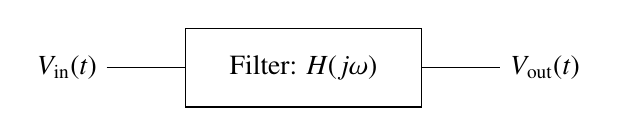
\begin{tikzpicture}
    % Draw the filter rectangle
    \draw (0,0) rectangle (3,1) node[midway] {Filter: $H(j\omega)$};
    
    % Draw the input and output labels
    \draw (-1,0.5) node[left] {$V_{\text{in}}(t)$} -- (0,0.5);
    \draw (3,0.5) -- (4,0.5) node[right] {$V_{\text{out}}(t)$};
\end{tikzpicture}
    \caption{Filter Equivalent of Circuit}
    \label{fig:2_gate.22.ee.31}
\end{figure}
\begin{align}
    H(j\omega) &= \brak{\frac{\sqrt{1 + 100\omega^2 C^2}}{2\sqrt{1 + 121\omega^2 C^2}}}e^{j(\tan^{-1}(10\omega C) - \tan^{-1}(11\omega C))}\\
    &= \brak{\frac{\sqrt{1 + 100\omega^2 C^2}}{2\sqrt{1 + 121\omega^2 C^2}}}e^{j\tan^{-1}\brak{\frac{-\omega C}{1 + 110\omega^2 C^2}}}\\
    \therefore V_{out}(t) &= 10\abs{H(j\omega)}\cos(\omega t + \angle H(j\omega))\\
    &= \frac{5\sqrt{1 + 100\omega^2 C^2}}{\sqrt{1 + 121\omega^2 C^2}}\cos\brak{\omega t -\tan^{-1}\brak{\frac{\omega C}{1 + 110\omega^2 C^2}}}
\end{align}
\begin{figure}[!h]
    \centering
    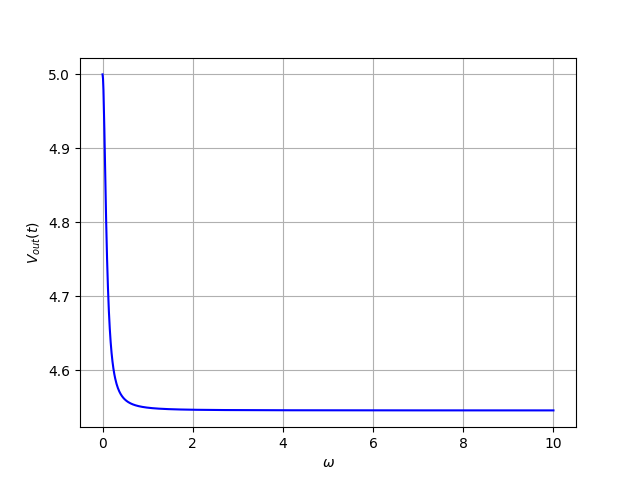
\includegraphics[width = \columnwidth]{2022/EE/31/figs/V_out_plot.png}
    \caption{Plot of $V_{out}(t)$ at $t=0$ w.r.t $\omega$}
    \label{fig:3_gate.22.ee.31}
\end{figure}

As $\omega \rightarrow 0$, $V_{in}(t)$ approaches being a D.C. input source ($10V$).

$\therefore$ substituting $\omega = 0$, we get:
\begin{align}
    V_{out}(t) &= 5V
\end{align}

%\end{document}


\pagebreak

\item An ideal OPAMP circuit with a sinusoidal input is shown in the figure. The 3dB frequency is the frequency at which the magnitude of the voltage gain decreases by 3 dB from the maximum value. Which of the options is/are correct?

\begin{figure}[H]
  \centering
  \input{2022/EC/26/codes/circuit1.tex}
  \label{fig:26fig1}
\end{figure}

\begin{enumerate}[label=(\Alph*)]
\item The circuit is a low pass filter.\\
\item The circuit is a high pass filter.\\
\item The 3 dB frequency is 1000rad/s.\\
\item The 3 dB frequency is $\frac{1000}{3}$rad/s.\\
\end{enumerate}
\hfill(GATE EC 2022)\\
\solution
\begin{center}
\begin{tikzpicture}
    % Box
    \draw (0,0) rectangle (4,2);

    % Arrow and label for x(t)
    \draw[->,>=stealth] (-1,1) -- node[above] {$x(t)$} (0,1);

    % Arrow and label for y(t)
    \draw[->,>=stealth] (4,1) -- node[above] {$y(t)$} (5,1);
\end{tikzpicture}
\end{center}

\pagebreak

\item A series $RLC$ circuit with $R = 10 \Omega$, $L = 50 mH$ and $C = 100 \micro F$ connected to
$200$ $V$, $50$ Hz supply consumes power $P$. The value of $L$ is changed such that this
circuit consumes same power $P$ but operates with lagging power factor. The new
value of L is $\hrulefill$ $mH$ (rounded off to two decimal places).
\hfill(GATE 33 BM 2022)

\solution
\iffalse
\let\negmedspace\undefined
\let\negthickspace\undefined
\documentclass[journal,12pt,twocolumn]{IEEEtran}
\usepackage{cite}
\usepackage{amsmath,amssymb,amsfonts,amsthm}
\usepackage{algorithmic}
\usepackage{graphicx}
\usepackage{textcomp}
\usepackage{xcolor}
\usepackage{txfonts}
\usepackage{listings}
\usepackage{enumitem}
\usepackage{mathtools}
\usepackage{gensymb}
\usepackage{comment}
\usepackage[breaklinks=true]{hyperref}
\usepackage{tkz-euclide} 
\usepackage{listings}
\usepackage{gvv}                                        
\def\inputGnumericTable{}                                 
\usepackage[latin1]{inputenc}                                
\usepackage{color}                                            
\usepackage{array}                                            
\usepackage{longtable}                                       
\usepackage{calc}                                             
\usepackage{multirow}                                         
\usepackage{hhline}                                           
\usepackage{ifthen}                                           
\usepackage{lscape}
\usepackage[center]{caption} % center the captions to figure

\newtheorem{theorem}{Theorem}[section]
\newtheorem{problem}{Problem}
\newtheorem{proposition}{Proposition}[section]
\newtheorem{lemma}{Lemma}[section]
\newtheorem{corollary}[theorem]{Corollary}
\newtheorem{example}{Example}[section]
\newtheorem{definition}[problem]{Definition}
\newcommand{\BEQA}{\begin{eqnarray}}
\newcommand{\EEQA}{\end{eqnarray}}
\newcommand{\define}{\stackrel{\triangle}{=}}
\theoremstyle{remark}
\newtheorem{rem}{Remark}
\begin{document}

\newcolumntype{M}[1]{>{\centering\arraybackslash}m{#1}}
\newcolumntype{N}{@{}m{0pt}@{}}

\bibliographystyle{IEEEtran}
\vspace{3cm}

\title{GATE 2022 BM 14 Q} 
\author{ee23btech11223 - Soham Prabhakar More% <-this % stops a space
}
\maketitle
\newpage
\bigskip

\renewcommand{\thefigure}{\theenumi}
\renewcommand{\thetable}{\theenumi}

\bibliographystyle{IEEEtran}

\textbf{Question:} $x\brak{t}$ is a real continuous-time signal whose magnitude frequency response
$\abs{X\brak{j\Omega}}$ is shown below. After sampling $x\brak{t}$ at 100 $rad.s^{-1}$, the spectral point P
is down-converted to \rule{1cm}{0.15mm} $rad.s^{-1}$ in the spectrum of the sampled signal.
\hfill{(GATE 2022 BM 14 Q)}
\begin{figure}[h!]
    \renewcommand\thefigure{1}
    \centering
    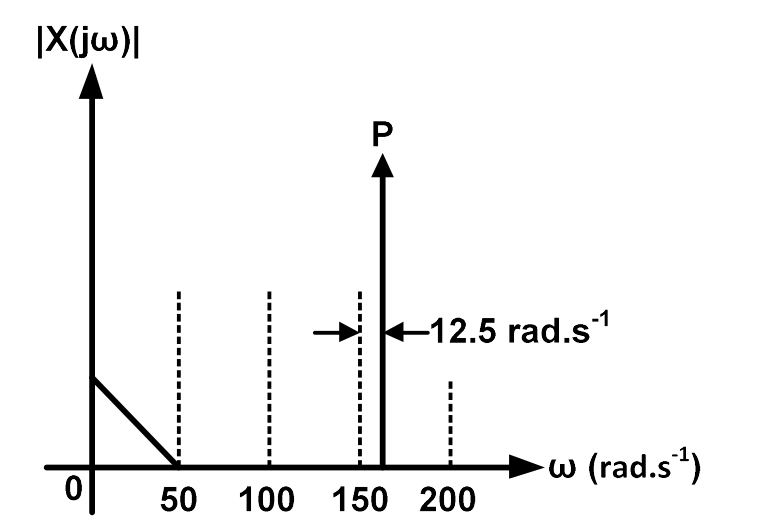
\includegraphics[width=\columnwidth]{2022/BM/14/figs/question.png}
    \caption[short]{Plot of $\abs{X\brak{j\omega}}$}
    \label{fig:2023.bm.14.img1}
\end{figure}

\solution
\fi
\begin{table}[ht]
    \renewcommand\thetable{1}
\begin{tabular}{|c|c|}
    \hline 
    \textbf{Parameter}&\textbf{Description} \\
    \hline
    $w\brak{t}$ & Sampling Function \\
    \hline
	$W\brak{j\omega}$ & Fourier Transform of $w\brak{t}$ \\
    \hline
    $x\brak{t}$ & Input Signal \\
    \hline
    $X\brak{j\omega}$ & Input Signal Frequency Spectrum \\
    \hline
    $x_s\brak{t}$ & Sampled Input Signal \\
    \hline
    $X_s\brak{j\omega}$ & Sampled Signal Frequency Spectrum \\
    \hline
\end{tabular}

\caption{Table of parameters}
\label{Table:1}


\end{table} \\
The sampling function is:
\begin{align}
    w(t) &= \sum_{k = -\infty}^{\infty}\delta\brak{t - \frac{2\pi k}{100}} \\
    W(j\omega) &= 100\sum_{k = -\infty}^{\infty}\delta\brak{j\brak{\omega - 100k}}
\end{align}
then the sampled function: 
\begin{align}
    x_s\brak{t} &= x\brak{t}w\brak{t} \\
    X_s\brak{j\omega} &= X\brak{j\omega} * W\brak{j\omega} \\
    X_s\brak{j\omega} &= \int_{-\infty}^{\infty}X\brak{j\theta}W\brak{j\brak{\omega - \theta}}d\theta \\
    X_s\brak{j\omega} &= 100\sum_{k = -\infty}^{\infty}\int_{-\infty}^{\infty}X\brak{j\theta}\delta\brak{j\brak{\omega - 100k - \theta}}d\theta \\
    X_s\brak{j\omega} &= 100\sum_{k = -\infty}^{\infty}X\brak{j\brak{\omega - 100k}} 
\end{align}
Thus, The down sampled point is at:
\begin{align}
    \omega &= \abs{162.5 - 100k}
\end{align}
where $k$ is the nearest integer to $\frac{162.5}{100}$, which is 2\\
Thus,
\begin{align}
    \omega = 37.5\,rad\,s^{-1}
\end{align}

\begin{figure}[h!]
    \renewcommand\thefigure{2}
    \centering
    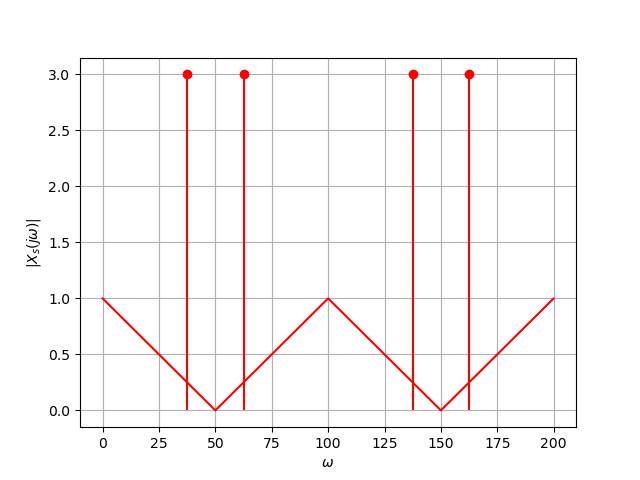
\includegraphics[width=\columnwidth]{2022/BM/14/figs/X_s.png}
    \caption[short]{Plot of $\abs{X_s\brak{j\omega}}$}
    \label{fig:2023.bm.14.img2}
\end{figure}

%\end{document}

\pagebreak

\item A single-phase full-bridge diode rectifier feeds a resistive load of $50 \Omega$ from a 200 V,
50 Hz single phase AC supply. If the diodes are ideal, then the active power, in watts,
drawn by the load is \rule{1cm}{0.5mm} (round off to nearest integer).  \\
\hfill (GATE EE 32)\\
\solution
\iffalse
\documentclass[journal,12pt,twocolumn]{IEEEtran}
\usepackage{amsmath,amssymb,amsfonts,amsthm}
\usepackage{txfonts}
\usepackage{tkz-euclide}
\usepackage{listings}
\usepackage{gvv}
\usepackage[latin1]{inputenc}
\usepackage{adjustbox}
\usepackage{array}
\usepackage{tabularx}
\usepackage{pgf}
\usepackage{lmodern}
\usepackage{circuitikz}
\usepackage{tikz}
\usepackage{graphicx}
\usepackage[english]{babel}

\begin{document}
\bibliographystyle{IEEEtran}

\vspace{3cm}

\title{}
\author{EE23BTECH11047 - Deepakreddy P
}
\maketitle
\newpage
\bigskip

\noindent \textbf{32} \quad A single-phase full-bridge diode rectifier feeds a resistive load of $50 \Omega$ from a 200 V,
50 Hz single phase AC supply. If the diodes are ideal, then the active power, in watts,
drawn by the load is \rule{1cm}{0.5mm} (round off to nearest integer).  \\
\hfill (GATE EE 32)\\
\solution\\
\fi

\begin{figure}[ht]
  \centering
      \begin{circuitikz}[american]
   \draw (0,8) to [sV=200V](0,-1) to [short](6,-1) to [short](6,0) to [D,l=$D_3$](9,3);
   \draw (0,8) to [short](6,8) to [short](6,6);
   \draw (6,6) to [D,l=$D_1$](9,3);
   \draw (3,3) to [D,l=$D_4$](6,6);
   \draw (3,3) to [D,l=$D_2$](6,0);
   \draw (3,3) to [short](2.5,3) to [crossing, bipoles/crossing/size=1](2.5,-4.8) to [short](12,-4.8) to [R=50$\Omega$](12,3) to [short](9,3);
   \draw (9,3) to [short,i=\Large{I}](12,3);
\end{circuitikz}

  \caption{Circuit-1}
\end{figure}

\begin{figure}[ht]
   \centering
   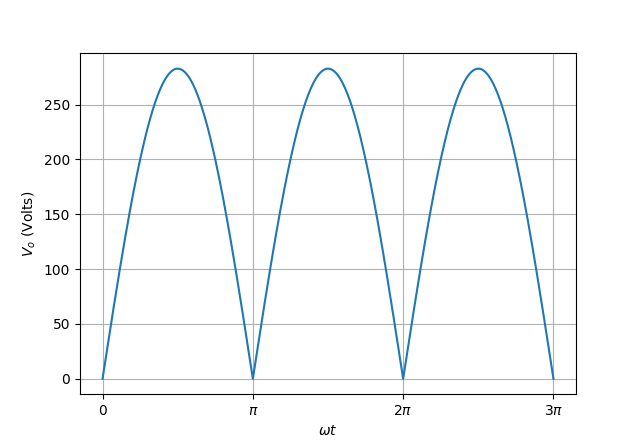
\includegraphics[width=1.2\columnwidth]{2022/EE/32/figs/gt1.png}
   \caption{Output voltage waveform of single-phase full
bridge rectifier}
\end{figure}


\begin{center}
    \begin{table}[ht]
        \setlength{\arrayrulewidth}{0.3mm}
\setlength{\tabcolsep}{12pt}
\renewcommand{\arraystretch}{1.3}


\begin{center}
\caption{Input Parameters}
\begin{tabular}{ |p{1.7cm}|p{1.7cm}|p{1.7cm}|  }

\hline
 {Symbol}&{Description} & {value}\\
\hline
R & Load Resistance & 50$\Omega$\\
\hline
$V_{rms}$ & RMS Voltage  & 200V\\
\hline
f & Frequency & 50Hz \\
\hline

\end{tabular}
\end{center}

    \end{table}
\end{center}

\begin{align}
    V_{rms} &= 200\\
    P &= \frac{\brak{V_{rms}}^2}{R}\\
    P &= \frac{\brak{200}^2}{50}W\\
    P &= 800W
\end{align}


%\end{document}


\pagebreak

\item The circuit shown is driven by a sinusoidal input voltage, $V_{\text{in}}$, resulting in the output voltage $V_{\text{out}}$. The frequency (in kilohertz) at which the voltage gain is 0 dB is (rounded off to two decimal places).
\begin{figure}[htb]
  \centering
  
\begin{circuitikz}
\tikzstyle{every node}=[font=\Large]
\draw [](10,10.5) to[short] (10,12.75);
\draw [](12.5,10.5) to[short] (12.5,12.75);
\draw (10,12.75) to[C] (12.5,12.75);
\draw (10.625,8.5) node[ieeestd buffer port, anchor=in](port){} (port.out) to[short] (12.25,8.5); \draw (port.in) to[short] (10.5,8.5);
\draw [](12.25,8.5) to[short, -o] (14.5,8.5);
\draw [](12.5,10.5) to[short] (12.5,8.5);
\draw [](11.25,9.75) to[short] (11.25,8.75);
\draw [](11.25,8.25) to[short] (11.25,7);
\draw [short] (10.75,8.5) -- (8.5,8.5);
\draw[] (11,8.25) to[short] (10,8.25);
\draw (10,8.25) to (10,7.25) node[ground]{};
\draw [](10,10.5) to[short] (10,8.5);
\draw (7,8.5) to[sinusoidal voltage source, sources/symbol/rotate=auto,l={ \LARGE $Vin$}] (7,6);
\draw (7,6) to (7,5.75) node[ground]{};
\node [font=\Large] at (11,13.5) {1 nF};
\node [font=\Large] at (5.75,7.25) {};
\node [font=\Large] at (15,8) {Vout};
\node [font=\Large] at (11.5,7.25) {-};
\node [font=\Large] at (11.5,9.75) {+};
\draw (10,10.75) to[R,l={ \Large $100k$}] (12.5,10.75);
\draw (7,8.5) to[R,l={ \Large $10k$}] (8.5,8.5);
\end{circuitikz}


\end{figure}
\hfill(GATE IN 2022)\\
\solution
\iffalse
\documentclass[journal,12pt,twocolumn]{IEEEtran}
\usepackage{cite}
\usepackage{amsmath,amssymb,amsfonts,amsthm}
\usepackage{algorithmic}
\usepackage{graphicx}
\usepackage{textcomp}
\usepackage{xcolor}
\usepackage{txfonts}
\usepackage{listings}
\usepackage{enumitem}
\usepackage{mathtools}
\usepackage{gensymb}
\usepackage{comment}
\usepackage[breaklinks=true]{hyperref}
\usepackage{tkz-euclide}
\usepackage{braket}
\def\inputGnumericTable{}
\usepackage[latin1]{inputenc}
\usepackage{color}
\usepackage{array}
\usepackage{longtable}
\usepackage{calc}
\usepackage{multirow}
\usepackage{hhline}
\usepackage{ifthen}
\usepackage{lscape}
\usepackage{gvv} 
\usepackage{circuitikz}

\newtheorem{theorem}{Theorem}[section]
\newtheorem{problem}{Problem}
\newtheorem{proposition}{Proposition}[section]
\newtheorem{lemma}{Lemma}[section]
\newtheorem{corollary}[theorem]{Corollary}
\newtheorem{example}{Example}[section]
\newtheorem{definition}[problem]{Definition}
\newcommand{\BEQA}{\begin{eqnarray}}
\newcommand{\EEQA}{\end{eqnarray}}
\newcommand{\define}{\stackrel{\triangle}{=}}
\theoremstyle{remark}
\newtheorem{rem}{Remark}

\begin{document}

\bibliographystyle{IEEEtran}
\vspace{3cm}

\title{GATE 2022 IN-56}
\author{EE23BTECH11201 - Abburi Tanusha$^{*}$% <-this % stops a space
}
\maketitle
\newpage
\bigskip

\renewcommand{\thefigure}{\theenumi}
\renewcommand{\thetable}{\theenumi}

\vspace{3cm}

\maketitle
\textbf{Question:} 
The circuit shown is driven by a sinusoidal input voltage, $V_{\text{in}}$, resulting in the output voltage $V_{\text{out}}$. The frequency (in kilohertz) at which the voltage gain is 0 dB is (rounded off to two decimal places).
\begin{figure}[htb]
	\centering
	
\begin{circuitikz}
\tikzstyle{every node}=[font=\Large]
\draw [](10,10.5) to[short] (10,12.75);
\draw [](12.5,10.5) to[short] (12.5,12.75);
\draw (10,12.75) to[C] (12.5,12.75);
\draw (10.625,8.5) node[ieeestd buffer port, anchor=in](port){} (port.out) to[short] (12.25,8.5); \draw (port.in) to[short] (10.5,8.5);
\draw [](12.25,8.5) to[short, -o] (14.5,8.5);
\draw [](12.5,10.5) to[short] (12.5,8.5);
\draw [](11.25,9.75) to[short] (11.25,8.75);
\draw [](11.25,8.25) to[short] (11.25,7);
\draw [short] (10.75,8.5) -- (8.5,8.5);
\draw[] (11,8.25) to[short] (10,8.25);
\draw (10,8.25) to (10,7.25) node[ground]{};
\draw [](10,10.5) to[short] (10,8.5);
\draw (7,8.5) to[sinusoidal voltage source, sources/symbol/rotate=auto,l={ \LARGE $Vin$}] (7,6);
\draw (7,6) to (7,5.75) node[ground]{};
\node [font=\Large] at (11,13.5) {1 nF};
\node [font=\Large] at (5.75,7.25) {};
\node [font=\Large] at (15,8) {Vout};
\node [font=\Large] at (11.5,7.25) {-};
\node [font=\Large] at (11.5,9.75) {+};
\draw (10,10.75) to[R,l={ \Large $100k$}] (12.5,10.75);
\draw (7,8.5) to[R,l={ \Large $10k$}] (8.5,8.5);
\end{circuitikz}


\end{figure}
\hfill(GATE IN 2022)\\
\textbf{Solution:} 
\fi

This circuit is an inverting OP-AMP. The transfer function of an inverting OP-AMP is given by\\
\begin{table}[h]
 	\centering
 	\resizebox{14 cm}{!}{
 		
\begin{tabular}{|c|c|c|}
\hline
\textbf{Parameter} &  \textbf{Value} & \textbf{Description} \\
\hline
 $20 \log \brak{\frac{V_{\text{out}}}{V_{\text{in}}}}$ & $0$ &Voltage gain\\
\hline
 Sinusoidal input voltage & $V_{\text{in}}$ & Input voltage applied to the circuit \\
\hline
 Output voltage & $V_{\text{out}}$ & Voltage across the output of the circuit \\
\hline
$R_1$ & 10 k$\Omega$ & Resistor connected to the inverting input of the OP-AMP \\
\hline
$R_2$ & 100 k$\Omega$ & Feedback resistor connected from the output to the inverting input of the OP-AMP \\
\hline
$C$ & 1 nF & Capacitor connected in parallel with $R_2$ \\
 \hline
 $Z_1$ &  ? & Impedance of resistor $R_1$ \\
 \hline
$Z_2$ & ? & Impedance of capacitor $C$ in series with resistor $R_2$ \\
\hline
\end{tabular}



 	}
 	\vspace{6 pt}
 	\caption{Parameters}
 \end{table}
\begin{align}
Z_1 &= R_1 \\
Z_2 &= \frac{R_2}{1+j \omega R_2C} \\
\frac{1}{Z_2} &= \frac{1}{R_2} + j\omega C \\
\frac{V_{\text{out}}}{V_{\text{in}}} &= -\frac{Z_2}{Z_1} \\
\frac{|V_{\text{out}}|}{|V_{\text{in}}|} &= \frac{|Z_2|}{|Z_1|} 
\end{align}
\begin{align}
20 \log \brak{\frac{V_{\text{out}}}{V_{\text{in}}}} &= 0 \\
\frac{V_{\text{out}}}{V_{\text{in}}} &= 1
\end{align}

\begin{align}
\frac{|V_{\text{out}}|}{|V_{\text{in}}|} &= \frac{|R_2|}{|(1+ j\omega R_2C)R_1|} = 1 \\
\frac{R_2}{R_1} &= \sqrt{1 + \brak{R_2 \omega C}^2} \\
10 &= \sqrt{1 + \brak{10^5 \cdot \omega 10^-9}^2} \\
99 &= \omega^2 \times 10^{-8} \\
\omega &= \sqrt{99} \times 10^4 \\
2\pi f &= 99.49 \times 10^3 \\
f &= 15.84 \, \text{kHz}
\end{align}
\begin{figure}[h!]
\centering
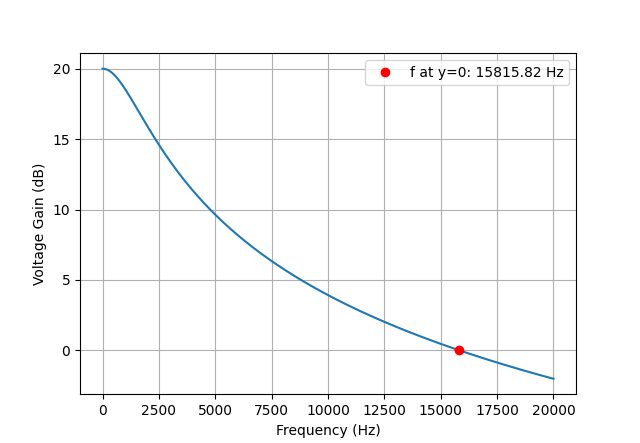
\includegraphics[width=\columnwidth]{2022/IN/56/figs/plot.png}
\caption{Frequency vs Voltage gain}
\end{figure}

%\end{document}

\pagebreak

\item An inductor having a $Q$-factor of 60 is connected in series with a capacitor having a $Q$-factor of 240. The overall $Q$-factor of the circuit is \_\_\_\_\_\_\_\_\_\_. (Round off to the nearest integer) \\
\hfill Gate 2022 EE Question 27\\
\solution
\iffalse
\let\negmedspace\undefined
\let\negthickspace\undefined
\documentclass[journal,12pt,twocolumn]{IEEEtran}
\usepackage{cite}
\usepackage{amsmath,amssymb,amsfonts,amsthm}
\usepackage{algorithmic}
\usepackage{graphicx}
\usepackage{textcomp}
\usepackage{xcolor}
\usepackage{txfonts}
\usepackage{listings}
\usepackage{enumitem}
\usepackage{mathtools}
\usepackage{gensymb}
\usepackage{comment}
\usepackage[breaklinks=true]{hyperref}
\usepackage{tkz-euclide} 
\usepackage{listings}                                   
\def\inputGnumericTable{}                                 
\usepackage[latin1]{inputenc}                                
\usepackage{color}                                            
\usepackage{array}                                            
\usepackage{longtable}                                       
\usepackage{calc}  
\usepackage{circuitikz}                                           
\usepackage{multirow}                                         
\usepackage{hhline}                                           
\usepackage{ifthen}                                           
\usepackage{lscape}
\newtheorem{theorem}{Theorem}[section]
\newtheorem{problem}{Problem}
\newtheorem{proposition}{Proposition}[section]
\newtheorem{lemma}{Lemma}[section]
\newtheorem{corollary}[theorem]{Corollary}
\newtheorem{example}{Example}[section]
\newtheorem{definition}[problem]{Definition}
\newcommand{\BEQA}{\begin{eqnarray}}
\newcommand{\EEQA}{\end{eqnarray}}
\newcommand{\define}{\stackrel{\triangle}{=}}
\newcommand{\brak}[1]{\langle #1 \rangle}
\theoremstyle{remark}
\newtheorem{rem}{Remark}

\begin{document}
\bibliographystyle{IEEEtran}
\vspace{3cm}
\title{\textbf{GATE 2022 EE}}
\author{EE23BTECH11023-ABHIGNYA GOGULA}
\maketitle
\newpage
\bigskip
\renewcommand{\thefigure}{\theenumi}
\renewcommand{\thetable}{\theenumi}
\textbf{Question27:}
\\An inductor having a $Q$-factor of 60 is connected in series with a capacitor having a $Q$-factor of 240. The overall $Q$-factor of the circuit is \_\_\_\_\_\_\_\_\_\_. (Round off to the nearest integer) \\
\hfill Gate 2022 EE Question 27\\
\section*{Solution}
\fi
\begin{circuitikz}
    \draw (0,0) to[R, l=$R_1$] (2,0) to[L, l=$L$] (4,0);
\end{circuitikz}
\begin{align}
Q_1=\frac{\omega_0 L}{R_1}
\end{align}
\begin{circuitikz}
    \draw (0,0) to[R, l=$R_2$] (2,0) to[C, l=$C$] (4,0);
\end{circuitikz}
\begin{align}
Q_2=\frac{1}{\omega_0 C R_2}
\end{align}
at resonance as $\omega_0 L =\frac{1}{\omega_0 C}$ hence
\begin{align}
Q_2=\frac{\omega_0 L}{R_2}
\end{align}
\begin{circuitikz}
    \draw (0,0) to[R, l=$R_1$] (2,0) to[L, l=$L$] (4,0) to[R, l=$R_2$] (6,0) to[C, l=$C$] (8,0);
\end{circuitikz}
\begin{align}
Q = \frac{\omega_0 L}{R_1+R_2}\\
Q = \frac{1}{\frac{R_1}{\omega_0 L}+\frac{R_2}{\omega_0 L}}
\end{align}
\begin{equation}
Q =\frac{Q_1 Q_2}{Q_1+Q_2}
\label{eq:EE 27eq1}
\end{equation}
then from \eqref{eq:EE 27eq1}
\begin{align}
Q=\frac{60 \times 240}{60+240}\\
Q=48
\end{align}
%\end{document}

\pagebreak

\item In the circuit shown, the switch is initially closed. It is opened at t= 0 s and
remains open thereafter. The time (in milliseconds) at which the output voltage
$V_{out}$ becomes LOW is  (round off to three decimal places)\hfill(GATE IN 2022)\\
\input{2022/IN/64/figs/tikzque}
\solution\\
\iffalse
\documentclass[journal,12pt,twocolumn]{IEEEtran}
\usepackage{amsmath,amssymb,amsfonts,amsthm}
\usepackage{txfonts}
\usepackage{tkz-euclide}
\usepackage{listings}
\usepackage{gvv}
\usepackage[latin1]{inputenc}
\usepackage{adjustbox}
\usepackage{array}
\usepackage{tabularx}
\usepackage{pgf}
\usepackage{lmodern}
\usepackage{circuitikz}
\usepackage{tikz}
\usepackage{graphicx}
\usepackage[english]{babel}

\begin{document}
\bibliographystyle{IEEEtran}

\vspace{3cm}

\title{}
\author{EE23BTECH11047 - Deepakreddy P
}
\maketitle
\newpage
\bigskip

\noindent \textbf{32} \quad An analog signal is sampled at 100 MHz to generate 1024 samples. Only
these samples are used to evaluate 1024-point FFT. The separation between
adjacent frequency points ($\Delta$F) in FFT is \rule{1cm}{0.5mm} kHz.\\
\hfill (GATE BM 2021)\\
\solution
\fi

\begin{center}
    \begin{table}[ht]
        \setlength{\arrayrulewidth}{0.3mm}
\setlength{\tabcolsep}{12pt}
\renewcommand{\arraystretch}{1.3}


\begin{center}
\caption{Input Parameters}
\begin{tabular}{ |p{1.7cm}|p{1.7cm}|p{1.7cm}|  }

\hline
 {Symbol}&{Description} & {value}\\
\hline
$f_s$ & Sampling frequency & 100 MHz\\
\hline
$N$ & No of samples  & 1024\\
\hline

\end{tabular}
\end{center}

    \end{table}
\end{center}

\begin{align}
    \Delta F &= \frac{f_s}{N}\\
    \Delta F &= \frac{100}{1024} MHz\\
    \Delta F &= \frac{10^5}{1024} kHz\\
    \Delta F &= 97.66kHz
\end{align}


\begin{figure}[ht]
   \centering
   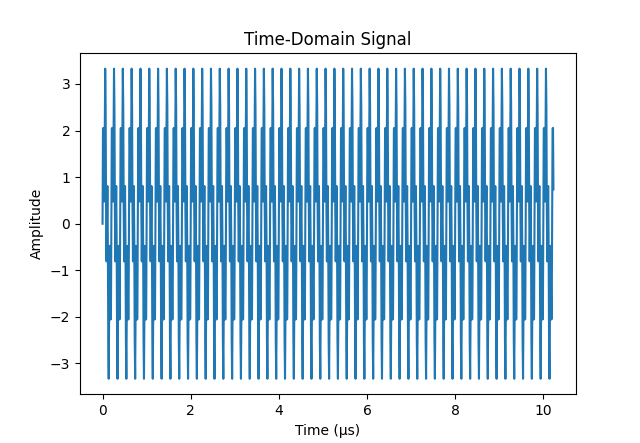
\includegraphics[width=1.1\columnwidth]{2021/BM/32/figs/fig1.png}
   \caption{Time Domain Signal}
\end{figure}

\begin{figure}[ht]
   \centering
   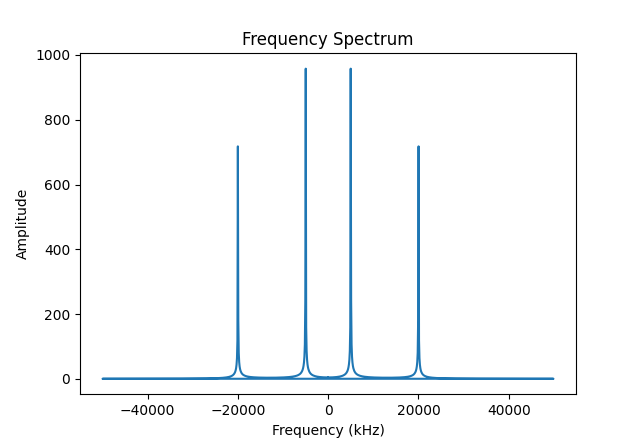
\includegraphics[width=1.1\columnwidth]{2021/BM/32/figs/fig2.png}
   \caption{Frequency Spectrum}
\end{figure}






%\end{document}


\pagebreak
\item For the Op-Amp circuit shown below, choose the correct output waveform corresponding to the input \( V_{\text{in}} = 1.5 \sin(20 \pi t) \) (in Volts). The saturation voltage for this circuit is \( V_{\text{sat}} = \pm 10 \) V.
\begin{figure}[ht]
\centering
    
\begin{circuitikz}
\tikzstyle{every node}=[font=\large]
\draw [, line width=0.7pt](11.5,9.75) node[op amp,scale=1] (opamp2) {}; \draw [, line width=0.7pt](opamp2.+) to[short] (10,9.25); \draw [, line width=0.7pt] (opamp2.-) to[short] (10,10.25); \draw [, line width=0.7pt](12.7,9.75) to[short](13,9.75);
\draw [](10,10.25) to[short] (10,10.5);
\draw [](10,11) to[short] (10,10.5);
\draw[] (10,11) to[short] (6.75,11);
\draw [, line width=0.9pt](6.75,11) to[sinusoidal voltage source, sources/symbol/rotate=auto,l={ \large $V_{in}$}] (6.75,8.5);
\draw [line width=0.9pt](6.75,8.5) to (6.75,8.25) node[ground]{};
\draw [, line width=0.9pt](10,4.75) to[resistor , i=$I_1$] (10,8.25);
\draw [, line width=0.9pt](10,8.25) to[resistor , i=$I_2$] (14.25,8.25);
\draw [, line width=0.9pt](12.75,9.75) to[short] (13.75,9.75);
\draw [, line width=0.9pt](10,8.25) to[short] (10,9.25);
\draw [, line width=0.9pt](13.75,9.75) to[short] (14.25,9.75);
\draw [, line width=0.9pt](14.25,9.75) to[short] (14.25,8.25);
\draw [line width=0.9pt](10,5) to (10,4.75) node[ground]{};
\node [font=\large] at (13,10) {$V_{out}$};
\node [font=\large] at (12.25,7.5) {$20k\Omega$};
\node [font=\large] at (9,6.75) {$2.2k\Omega$};
\end{circuitikz}


\end{figure}
\begin{enumerate}
  \item[(A)]
  \begin{figure}[ht!]
    \centering
    
\begin{circuitikz}
\tikzstyle{every node}=[font=\small]

\draw [](8.75,9.75) to[short] (8.75,13.25);
\draw[, line width=0.5pt] (8.75,10) to[short] (8.5,10);
\draw[, line width=0.5pt] (8.75,10.75) to[short] (8.5,10.75);
\draw[, line width=0.5pt] (8.75,11.5) to[short] (8.5,11.5);
\draw[, line width=0.5pt] (8.75,12.25) to[short] (8.5,12.25);
\draw[, line width=0.5pt] (8.75,13) to[short] (8.5,13);
\node [font=\small] at (11,9.5) {Time };
\node [font=\small] at (8.25,13) {10};
\node [font=\small] at (8.25,12.25) {5};
\node [font=\small] at (8.25,11.5) {0};
\draw[, line width=0.5pt] (12.5,9.75) to[short] (8.75,9.75);
\draw [, line width=0.5pt](8.75,13) to[short] (9,13);
\draw [, line width=0.5pt](9,13) to[short] (9,10);
\draw [, line width=0.5pt](9,10) to[short] (9.75,10);
\draw [, line width=0.5pt](9.75,10) to[short] (9.75,13);
\draw [, line width=0.5pt](9.75,13) to[short] (10.5,13);
\draw [, line width=0.5pt](10.5,13) to[short] (10.5,10);
\draw [, line width=0.5pt](10.5,10) to[short] (11.25,10);
\draw [, line width=0.5pt](11.25,10) to[short] (11.25,13);
\draw [, line width=0.5pt](11.25,13) to[short] (12,13);
\draw [, line width=0.5pt](12,13) to[short] (12,10);
\draw [, line width=0.5pt](12,10) to[short] (12.5,10);
\node [font=\small] at (8.25,10.75) {-5};
\node [font=\small] at (8.25,10) {-10};
\node [font=\small] at (7.75,11) {$V_{out}$\brak{volts}};
\end{circuitikz}

\end{figure}
  \item[(B)]  
  \begin{figure}[ht]
    \centering
    
\begin{circuitikz}
\tikzstyle{every node}=[font=\small]

\draw [](8.75,9.75) to[short] (8.75,13.25);
\draw[, line width=0.5pt] (8.75,10) to[short] (8.5,10);
\draw[, line width=0.5pt] (8.75,10.75) to[short] (8.5,10.75);
\draw[, line width=0.5pt] (8.75,11.5) to[short] (8.5,11.5);
\draw[, line width=0.5pt] (8.75,12.25) to[short] (8.5,12.25);
\draw[, line width=0.5pt] (8.75,13) to[short] (8.5,13);
\node [font=\small] at (11,9.5) {Time };
\node [font=\small] at (8.25,13) {10};
\node [font=\small] at (8.25,12.25) {5};
\node [font=\small] at (8.25,11.5) {0};
\draw[, line width=0.5pt] (12.5,9.75) to[short] (8.75,9.75);
\draw [, line width=0.5pt](8.75,13) to[short] (12.5,13);
\node [font=\small] at (8.25,10.75) {-5};
\node [font=\small] at (8.25,10) {-10};
\node [font=\small] at (7.75,11) {$V_{out}$(volts)};
\end{circuitikz}

\end{figure}
  \item[(C)] 
  \begin{figure}[ht]
    \centering
    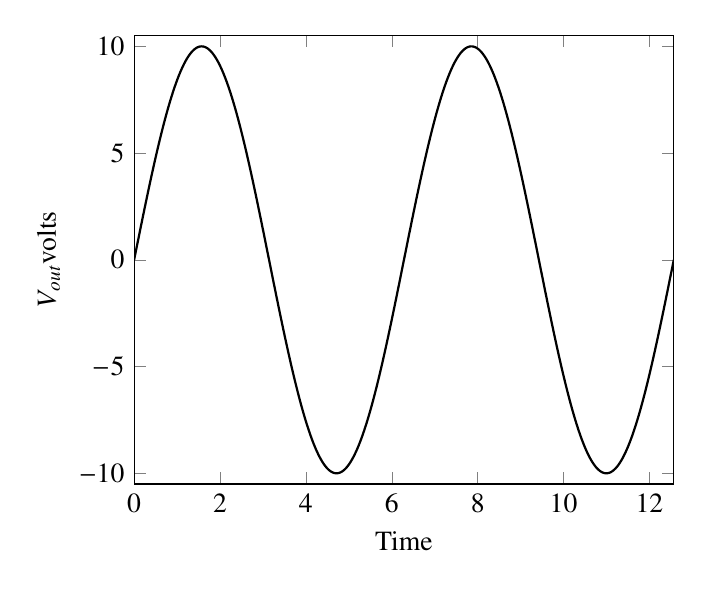
\begin{tikzpicture}
\begin{axis}[
    xlabel=Time,
    ylabel={$V_{out}$\brak{volts}},
    xmax=4*pi, xmin=0, 
    ymax=10.5, ymin=-10.5, % Adjust these values according to your data range
    ytick={-10,-5,0,5,10}, % Adjust these values according to your data range
    yticklabels={$-10$,$-5$,$0$,$5$,$10$}, % Adjust these values according to your data range
]
\addplot[domain=0:4*pi, samples=400, black, thick]{10*sin(deg(x))};
\end{axis}
\end{tikzpicture}

\end{figure}
  \item[(D)] 
   \begin{figure}[ht]
    \centering
    \begin{circuitikz}
\tikzstyle{every node}=[font=\small]
\draw [](8.75,9.75) to[short] (8.75,13.25);
\draw[, line width=0.5pt] (8.75,10) to[short] (8.5,10);
\draw[, line width=0.5pt] (8.75,10.75) to[short] (8.5,10.75);
\draw[, line width=0.5pt] (8.75,11.5) to[short] (8.5,11.5);
\draw[, line width=0.5pt] (8.75,12.25) to[short] (8.5,12.25);
\draw[, line width=0.5pt] (8.75,13) to[short] (8.5,13);
\node [font=\small] at (11,9.5) {Time };
\node [font=\small] at (8.25,13) {10};
\node [font=\small] at (8.25,12.25) {5};
\node [font=\small] at (8.25,11.5) {0};
\draw [, line width=0.5pt](8.75,11.5) to[short] (12.5,11.5);
\draw[, line width=0.5pt] (12.5,9.75) to[short] (8.75,9.75);
\node [font=\small] at (8.25,10.75) {-5};
\node [font=\small] at (8.25,10) {-10};
\node [font=\small] at (7.75,11.25) {$V_{out}$(volts)};
\end{circuitikz}

\end{figure}
\end{enumerate}

\hfill{(GATE PH 2022)}\\
\solution
\end{enumerate}
